\documentclass[a4paper, oneside]{memoir}% Document class
\usepackage[a4paper]{geometry}			% Margins
\usepackage{lmodern}
\usepackage{graphicx}
\usepackage{float}
\usepackage{listings}
\usepackage[small,compact]{titlesec}	% No 'chapter' in chapter headings.
\graphicspath{{Media/}}					% Directory that holds images.

\titleformat{\chapter}[hang]
{\normalfont\Large\bfseries}{\thechapter}{1em}{\Large}
\titlespacing{\chapter}{0pt}{*0}{*1}

\titleformat{\chapter}{\Huge\bfseries}{\thechapter}{1em}{}
\titleformat{\section}{\LARGE\bfseries}{\thesection}{1em}{}
\titleformat{\subsection}{\Large\bfseries}{\thesubsection}{1em}{}
\titleformat{\subsubsection}{\normalsize\bfseries}{\thesubsubsection}{1em}{}

\usepackage{subcaption}

\author{
  Erik Sidelmann Jensen\\
  \texttt{ejens11@student.aau.dk}
  \and
  Lasse Vang Gravesen\\
  \texttt{lgrave11@student.aau.dk}
  \and
  Dennis Jakobsen\\
  \texttt{djakob11@student.aau.dk}  
}

\title{Data Intensive Systems - Miniproject - Part 3}
\date{}

\begin{document}
	\clearpage\maketitle
	\thispagestyle{empty}
	
	\chapter{DIS Miniproject}
	\section{Task E \& F}
	We defined our multidimensional cube using the following xml:
	\lstinputlisting[language=XML]{fklubdw.xml}
	
	We then could answer the following questions:
	
	\textbf{How much is bought at some point during some day?}
	
	We can answer this by looking at summarized hours, we look at the hours with the most spent.
	
	28,618,675 Ører has been spent at the 12th hour and 20,400,875 Ører has been spent at the 13th hour.
	
	\textbf{How does the amount sold change over time?}
	We can answer this by looking at individual years and how much is total spent on each of the years.
	\begin{table}[H]
	    \begin{tabular}{l|l}
	    Year & Sale Amount \\ \hline
	    1996 & 187,650     \\
	    1997 & 2,359,375   \\
	    1998 & 13,696,025  \\
	    1999 & 15,180,275  \\
	    2000 & 15,763,800  \\
	    2001 & 16,402,075  \\
	    2002 & 19,679,050  \\
	    2003 & 18,017,550  \\
	    2004 & 19,876,325  \\
	    2005 & 17,882,675  \\
	    2006 & 20,225,450  \\
	    2007 & 19,932,050  \\
	    2008 & 61,650      \\
	    \end{tabular}
	\end{table}
	
	As it can be seen the first years had little sales compared to the later years such as 2002 through 2007. The last year presented 2008 may be an invalid
	year since the total sales may be misleading if sales for a whole year is not considered.

	\textbf{When is it best to restock, given low activity?}
	
	We can answer this by looking at which hours have the least activity during 8-16.
	
	Those hours are 8 with 9,632,450 and 16 with 9,981,050.
	
	A better way of answering this would be to look at the weekdays too, but we do not have that field.
	
	\textbf{Which product gives the most revenue?}
	\begin{table}[H]
	    \begin{tabular}{l|l}
	    Name               & Sale Amount \\ \hline
	    ½L Vand excl. pant & 66,970,550  \\
	    Øl                 & 20,272,250  \\
	    ½L Matilde cacao   & 19,476,750  \\
	    Kaffe/Choko(1 kop) & 11,578,400  \\
	    Juice              & 8,738,675   \\
	    \end{tabular}
	\end{table}
	
	\textbf{What does the increase in sale for specific products look like over time?}
	See Figure \ref{fig:yearProduct} for a graphical overview of how the sales for soda without deposit(pant), Matilde kakao, juice, and beer changes over each year. For example it can be seen that beer was a popular drink in 2002. The figure is split in a non-drilled version in Figure \ref{fig:yearProductNormal} and a drilled in Figure \ref{fig:yearProductDrilled}
	
	\begin{figure}
		\begin{subfigure}{.5\textwidth}
			\centering
			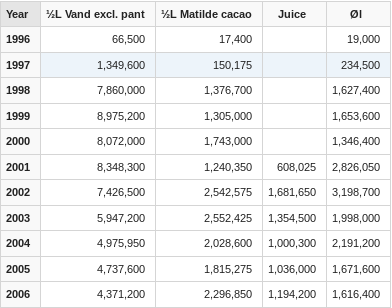
\includegraphics[scale=0.5]{year_productName.png}
			\caption{Normal version}
			\label{fig:yearProductNormal}
		\end{subfigure}
		\begin{subfigure}{.5\textwidth}
			\centering
			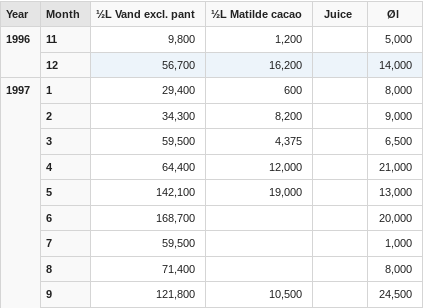
\includegraphics[scale=0.5]{drilldownMonthProduct.png}
			\caption{Drilled down version}
			\label{fig:yearProductDrilled}
		\end{subfigure}
		\caption{Different product sales over time.}
		\label{fig:yearProduct}
	\end{figure}
	
	\textbf{Is it worth it to sell soda without deposit(pant)}
	See Figure \ref{fig:sodaSales} for an illustration of how the sales are of soda with and without deposit(pant). It can for example be seen that the sale for soda with deposit(pant) is only a fraction of the sales of soda without. The figure is split in a non-sliced and sliced version in Figure \ref{fig:sodaSalesNormal} and Figure \ref{fig:sodaSalesSliced}
	
	\begin{figure}
		\begin{subfigure}{.5\textwidth}
			\centering
			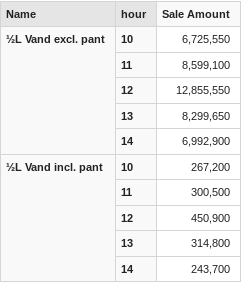
\includegraphics[scale=0.5]{product_hour_sales.png}
			\caption{Normal version}
			\label{fig:sodaSalesNormal}
		\end{subfigure}
		\begin{subfigure}{.5\textwidth}
			\centering
			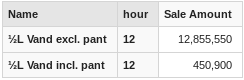
\includegraphics[scale=0.5]{drilldownProductHourSales.png}
			\caption{Slice and diced}
			\label{fig:sodaSalesSliced}
		\end{subfigure}
\caption{Sales of soda with and without deposit(pant)}
\label{fig:sodaSales}
	\end{figure}
	
	\textbf{Which member have spent the most?}
	The member that has spent the most is '1704' having spent 1,439,650 ører, see Figure \ref{fig:memberSales}.
	
	\begin{figure}
		\centering
		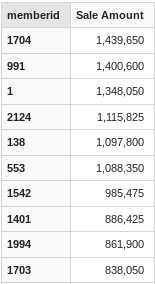
\includegraphics[scale=0.5]{member_sales.png}
		\caption{Member ids and sales}
		\label{fig:memberSales}
	\end{figure}
\end{document}
